\chapter{Моделирование роста трещин автоГРП в длину} \label{ch3}

\section{Постановка задачи}
\vspace*{-5mm}

На основе модели одномерных утечек Картера \cite{karter} в работе \cite{koning} получена первая формула Кёнинга, которая представляет собой зависимость полудлины трещины автоГРП от расхода жидкости, фильтрационно-ёмкостных свойств пласта, репрессии на пласт и времени:
\beq\label{Koning_first}
x_{\!f}=\frac{Q\mu\sqrt{\pi\kappa t}}{2\pi k_eh\left(p_{\!f}-p_e\right)},
\eeq
где $Q$ -- расход нагнетаемой в рассматриваемую трещину жидкости;
$\mu$ -- вязкость жидкости;
$\kappa=k_e/(\varphi_e\mu c_t)$ -- коэффициент пьезопроводности пласта;
$t$ -- время закачки;
$k_e$ -- проницаемость пласта;
$\varphi_e$ -- пористость пласта;
$c_t$ -- общая сжимаемость системы (состоит из сжимаемости флюидов и сжимаемости порового пространства);
$h$ -- эффективная толщина (мощность) пласта;
$\Delta p=p_{\!f}-p_e$ -- разница между средним давлением в трещине и пластовым давлением (репрессия на пласт).\\

В текущей работе рассматривается одновременный рост нескольких трещин гидроразрыва, поэтому расход жидкости на каждой из них может динамично меняться согласно правилам Кирхгофа.
Кроме того, давление в трещинах в общем случае тоже может меняться по мере увеличения объёма трещин и изменения расхода на них.
Получается, что согласно формуле \eqref{Koning_first} есть зависимость полудлины трещины $x_{\!f}$ от расхода на трещине $Q$, но при этом на расход в общем случае может влиять текущая полудлина каждой из трещин.

Таким образом, для корректного применения формулы Кёнинга приращение полудлины каждой из трещин на текущем шаге по времени необходимо найти как произведение полной производной формулы Кёнинга по времени и рассматриваемого временного шага.\newline
Полная производная полудлины трещины $x_{\!f}$ по времени $t$:
\beq\label{FullDerivative}
\frac{dx_{\!f}}{dt}=\frac{\partial x_{\!f}}{\partial t}+\frac{\partial x_{\!f}}{\partial Q}\frac{dQ}{dt}+\frac{\partial x_{\!f}}{\partial p_{\!f}}\frac{dp_{\!f}}{dt}
\eeq
Частная производная полудлины трещины $x_{\!f}$ по времени $t$:
\beq\label{PartialDerivative_t_first}
\frac{\partial x_{\!f}}{\partial t}=\frac{Q\mu}{4\pi k_eh\left(p_{\!f}-p_e\right)}\sqrt{\frac{\pi\kappa}{t}}
\eeq
Частная производная полудлины трещины $x_{\!f}$ по расходу $Q$:
\beq\label{PartialDerivative_Q_first}
\frac{\partial x_{\!f}}{\partial Q}=\frac{\mu\sqrt{\pi\kappa t}}{2\pi k_eh\left(p_{\!f}-p_e\right)}
\eeq
Частная производная полудлины трещины $x_{\!f}$ по репрессии на пласт $\left(p_{\!f}-p_e\right)$:
\beq\label{PartialDerivative_p_first}
\frac{\partial x_{\!f}}{\partial (p_{\!f}-p_e)}=-\frac{Q\mu\sqrt{\pi\kappa t}}{2\pi k_eh\left(p_{\!f}-p_e\right)^2}
\eeq
Подставляя \eqref{PartialDerivative_t_first}, \eqref{PartialDerivative_Q_first} и \eqref{PartialDerivative_p_first} в выражение \eqref{FullDerivative}, получаем:
\beq\label{FullDerivativeExplicit_first}
\frac{dx_{\!f}}{dt}=\frac{\mu}{2\pi k_e h(p_{\!f}-p_e)}\left(\frac{Q}{2}\sqrt{\frac{\pi\kappa}{t}}+\sqrt{\pi\kappa t}\,\frac{dQ}{dt}-\frac{Q\sqrt{\pi\kappa t}}{\left(p_{\!f}-p_e\right)}\frac{d(p_{\!f}-p_e)}{dt}\right)
\eeq
             
Итак, приращение полудлины трещины на каждом шаге по времени при рассмотрении случая одномерных утечек Картера записывается в следующем виде:
\beq\label{IncrementExplicit_first}
dx_{\!f}=\frac{\mu}{2\pi k_e h(p_{\!f}-p_e)}\left(\frac{Q}{2}\sqrt{\frac{\pi\kappa}{t}}dt+\sqrt{\pi\kappa t}\,dQ-\frac{Q\sqrt{\pi\kappa t}}{\left(p_{\!f}-p_e\right)}d(p_{\!f}-p_e)\right)
\eeq\\

Дополнительно в работе \cite{koning} получена вторая формула Кёнинга, которая применяется в случае двумерных радиальных утечек жидкости из трещины в пласт и представляет собой зависимость полудлины трещины автоГРП от расхода жидкости, фильтрационно-ёмкостных свойств пласта, репрессии на пласт и времени:
\beq\label{Koning_second}
x_{\!f}=3\exp{\!\left(-\frac{2\pi k_e h\left(p_{\!f}-p_e\right)}{Q\mu}\right)}\sqrt{\kappa t}
\eeq
В этом случае частная производная полудлины трещины $x_{\!f}$ по времени $t$:
\beq\label{PartialDerivative_t_second}
\frac{\partial x_{\!f}}{\partial t}=\frac{3}{2}\exp{\left(-\frac{2\pi k_e h \left(p_{\!f}-p_e\right)}{Q\mu}\right)}\sqrt{\frac{\kappa}{t}}
\eeq
Частная производная полудлины трещины $x_{\!f}$ по расходу $Q$:
\beq\label{PartialDerivative_Q_second}
\frac{\partial x_{\!f}}{\partial Q}=\frac{6\pi k_e h\left(p_{\!f}-p_e\right)}{Q^2\mu}\exp{\!\left(-\frac{2\pi k_e h\left(p_{\!f}-p_e\right)}{Q\mu}\right)}\sqrt{\kappa t}
\eeq
Частная производная полудлины трещины $x_{\!f}$ по репрессии на пласт $\left(p_{\!f}-p_e\right)$:
\beq\label{PartialDerivative_p_second}
\frac{\partial x_f}{\partial (p_{\!f}-p_e)}=-\frac{6\pi k_e h}{Q\mu}\exp{\!\left(-\frac{2\pi k_e h\left(p_{\!f}-p_e\right)}{Q\mu}\right)}\sqrt{\kappa t}
\eeq

Подставляя \eqref{PartialDerivative_t_second}, \eqref{PartialDerivative_Q_second} и \eqref{PartialDerivative_p_second} в выражение \eqref{FullDerivative}, получаем:
\beq
\begin{gathered}
\frac{dx_{\!f}}{dt}=\exp{\!\left(-\frac{2\pi k_e h\left(p_{\!f}-p_e\right)}{Q\mu}\right)}\left(\frac{3}{2}\sqrt{\frac{\kappa}{t}}\,+\right.\\[10pt]
+\left.\frac{6\pi k_e h\left(p_{\!f}-p_e\right)}{Q^2\mu}\sqrt{\kappa t}\,\frac{dQ}{dt}-\frac{6\pi k_e h}{Q\mu}\sqrt{\kappa t}\,\frac{d(p_{\!f}-p_e)}{dt}\right)
\end{gathered}
\eeq

Итак, приращение полудлины трещины на каждом шаге по времени при рассмотрении случая двумерных радиальных утечек жидкости из трещины в пласт записывается в следующем виде:
\beq\label{IncrementExplicit_second}
\begin{gathered}
dx_{\!f}=\exp{\!\left(-\frac{2\pi k_e h\left(p_{\!f}-p_e\right)}{Q\mu}\right)}\left(\frac{3}{2}\sqrt{\frac{\kappa}{t}}dt\,+\right.\\[10pt]
+\left.\frac{6\pi k_e h\left(p_{\!f}-p_e\right)}{Q^2\mu}\sqrt{\kappa t}\,dQ-\frac{6\pi k_e h}{Q\mu}\sqrt{\kappa t}\,d(p_{\!f}-p_e)\right)
\end{gathered}
\eeq

Постановка задачи принимает следующий вид: используя решатель уравнений Кирхгофа, реализованный в главе \ref{ch3}, и формулы для приращения полудлины трещины \eqref{IncrementExplicit_first} и \eqref{IncrementExplicit_second}, построить графики зависимостей полудлины трещины и расхода на трещинах от времени при одномерных утечках Картера и при двумерных радиальных утечках жидкости из трещины в пласт.

\section{Описание численного алгоритма решения}

Совмещение формулы Кёнинга с уравнениями Кирхгофа будет проведено следующим образом:

1) на текущем шаге по времени по имеющимся значениям полудлины трещин автоГРП предыдущего шага будут рассчитаны давления и расходы на каждой трещине;

2) на основе полученных значений приращения давления и расхода будет найдено приращение полудлины трещины $dx_{\!f}$ на данном временном шаге по формуле \eqref{2_7};

3) по формуле $x_{\!f}^{\text{current}}=x_{\!f}^{\text{last}}+dx_{\!f}$ будут найдены полудлины каждой из трещин на текущем временном шаге;

4) описанные действия будут проделаны до требуемого шага по времени (условия остановки).

%\section{Результаты моделирования}
%
%\begin{figure}[H]
%	\adjustbox{minipage=1.3em,valign=t}{\subcaption{}\label{fig:p_0(q_0)}}%
%	\begin{subfigure}[t]{\dimexpr.5\linewidth-1.3em\relax}
%		\centering
%		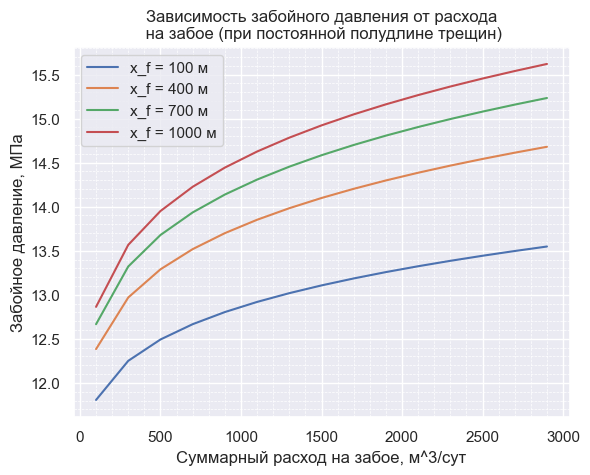
\includegraphics[width=.95\linewidth,valign=t]{images/p_0(q_0).png}
%	\end{subfigure}
%\hfill %выровнять по ширине
%	\adjustbox{minipage=1.3em,valign=t}{\subcaption{}\label{fig:p_0(x_f)}}%
%	\begin{subfigure}[t]{\dimexpr.5\linewidth-1.3em\relax}
%		\centering
%		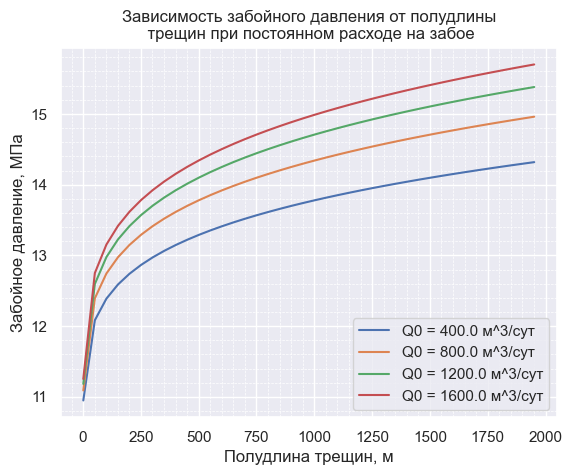
\includegraphics[width=.95\linewidth,valign=t]{images/p_0(x_f).png}
%	\end{subfigure}
%\captionsetup{justification=centering} %центрировать
%\caption{Зависимости забойного давления от основных параметров задачи: {\itshape a} --- от суммарного расхода на забое; {\itshape b} --- от полудлины трещин} 
%\label{fig:results1}
%\end{figure}

%Результаты моделирования представлены на рис. \ref{fig:results2}.
 
%\begin{figure}[H] 
%\center
%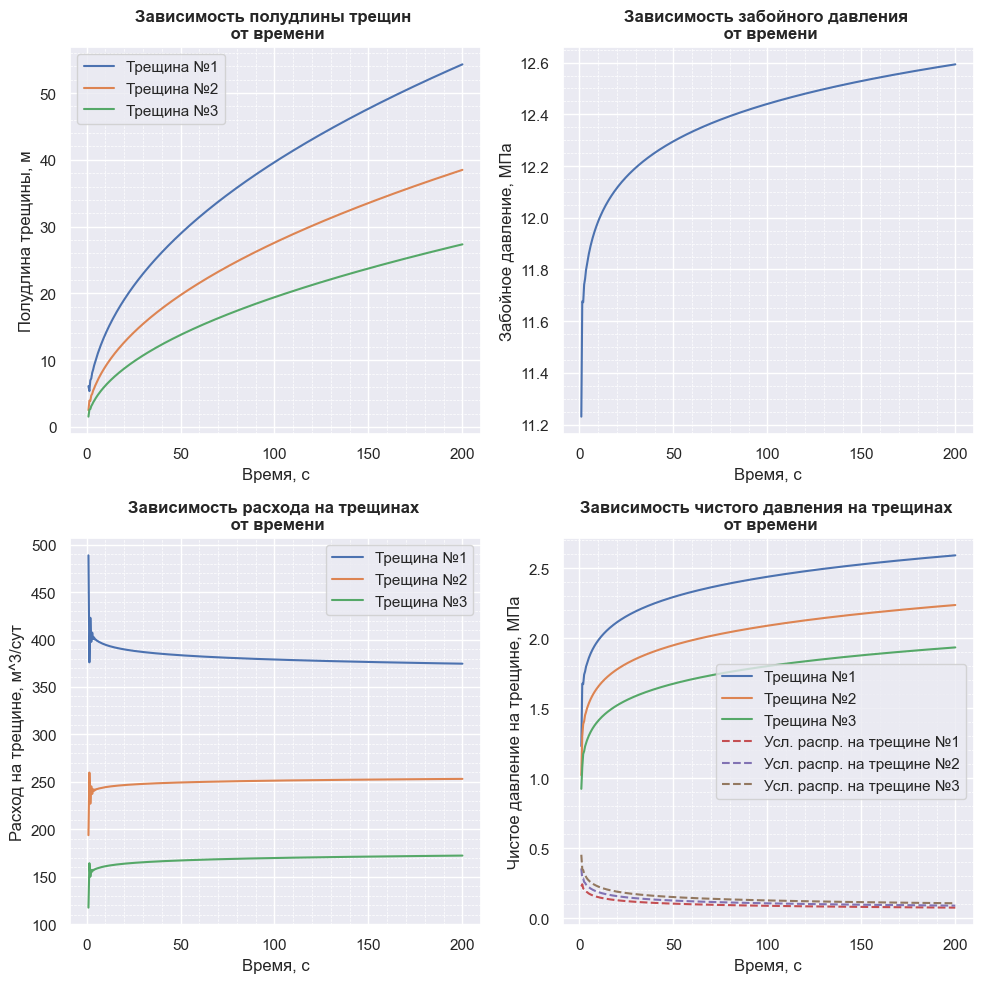
\includegraphics[width=.85\linewidth]{images/Kirchhoff+Koning.png}
%\caption{Результаты решения поставленной задачи} 
%\label{fig:results2}  
%\end{figure}

%В проведённом численном эксперименте трещины отличаются друг от друга количеством и диаметром перфораций.\newline
%У трещины 1: количество перфораций 32, диаметр перфораций 0.02 м.\newline
%У трещины 2: количество перфораций 2, диаметр перфораций 0.01 м.\newline
%У трещины 3: количество перфораций 1, диаметр перфораций 0.01 м.
%\\

%Код решения представлен по ссылке: \url{https://github.com/mualal/hydrofracturing/blob/master/notebooks/02_fractures_growth_with_Koning.ipynb}

%Из графиков на рис. \ref{fig:results2} видим, что большую часть потока забирает на себя трещина с лучшими перфорациями.
%Эта же трещина лидирует по скорости роста.

%Также видим, что при росте трещин требуется всё большее забойное давление для того, чтобы поддерживать этот рост.

%При выбранных входных параметрах построенной модели чистое давление в каждой из трещин существенно превышает давления критерия распространения, следовательно, при достаточно высоком забойном давлении все трещины будут расти одновременно.
